\documentclass[11 pt]{article}
\usepackage[a4paper]{geometry}
\usepackage{float}
\usepackage{multirow}    % to add multirow cells in tables
\usepackage{indentfirst} %to automatically intent the first paragrap of each sections
\usepackage{amsmath}		%math packages
\usepackage{mathtools}
\usepackage{amssymb}
\usepackage{graphicx}	%Required for inserting images
\usepackage{fontenc}
\usepackage[colorlinks=true,linkcolor=blue,citecolor=blue, urlcolor=blue]{hyperref}	%for hyperlinks
\usepackage{subcaption}	%to add subcaptions within single floating enviroments
\usepackage{placeins}	%to control position of floating enviroments
\usepackage[numbers]{natbib}  %for correct formating of bibliography}\usepackage{import}
\usepackage[utf8]{inputenc}
\usepackage{tikz}
\usepackage{tikz-cd}
\usepackage{pgfplots}
\pgfplotsset{compat=1.14}
\bibliographystyle{abbrvnat}
\usepackage{siunitx} %for correct formating of units



\textwidth=170mm
\textheight=250mm
\hoffset= -20mm       % may need change
\voffset= -25mm       % may need change


\begin{document}
\pagenumbering{roman}
%% we do the title page ourselves
\thispagestyle{empty}     % only for frontpage
\null\vspace{40mm}
\begin{center}
{%%%%%%%%%%%%%%%%%%%%%%%%%% Titel
\Large  
Studying the $Z$ Boson with the ATLAS Detector at the LHC \footnote{\noindent Experiment FP94 perfomed the $4^{\textrm{th}}$ Nov. 2024. Supervisor:	Ruiz, Miguel}
}\\[15mm]
%%%%%%%%%%%%%%%%%%%%%%%%%%% Authors
Q. Coc and P. Huth

\vspace{25mm}

\parbox{0.9\textwidth}{
\textbf{Abstract}:    
\small 
In this experiment we measure the mass and width of the $Z$-Boson using pre-selected data collected by the ATLAS detector at the LHC in 2012 along with Monte Carlo (MC) simulations of Standard Model processes [cite]. The comparison of both data sets, measurements and MC, reveal data points generated by secondary processes irrelevant for our purposes, which where consequently filtered out. By fitting the convolution of a Gaussian and a Breit-Wigner distribution to the filtered data we determine $m_{Z} = \SI{90.629\pm 0.005}{\giga\electronvolt}$ and $\Gamma = \SI{3.258\pm 0.021}{\giga\electronvolt}$. Both values display a significant deviation from the values reported by the Particle Data Group \footnotemark of $\sigma_{M_Z} = 27.11$ and $\sigma_{M_Z} = 36.09$.
}
\end{center}
\footnotetext{S. Navas et al. (Particle Data Group), Dec. 2024.\href{https://pdglive.lbl.gov/Particle.action?node=S044&init=0}{[Online]}}
\vfill
Als besondere Auswertung testiert: Datum, Unterschrift:
\vspace{20mm}

%% Rueckseite des Titelblatts leer. Bei einseitigem Druck entfernen
\newpage  
\null\thispagestyle{empty} 

\newpage
\pagenumbering{arabic}

\section{Introduction}
%
%Nowadays, physics describes matter and its interactions using the standard model of particles (SM). This field theory contains what are thought to be all of the elementary particles and the bosons that mediate three out of the four existing forces of nature. The theoretical framework has shown great success in describing a large number of phenomena. Among it main achievements, we find the unification of the  electromagnetic and weak forces united into one theory, the electro weak theory.

The electroweak theory, unification of the electromagnetic and weak forces, was developed during the 70's by S. Glashow, A. Salam and S. Weinberg. It's lagrangian is symmetric under  $SU(2)_{L}\times U_{Y}$ local gauge transformations and thus gives rise to 4 gauge bosons. After spontaneous symmetry breaking (SSB) the Goldstone-bosons corresponding to the weak interaction, $W^{+}$, $W^{-}$ and $Z$, acquire large masses while the boson mediating the electromagnetic, photon $\gamma$, remains massless. Five years after the publication of the electroweak theory, the $W^\pm$ and $Z$ boson were discovered experimentally.

The $W$ and $Z$ bosons were found at CERN. First, in the study of proton-antiproton collisions at the SPS and secondly in the analysis of electorn-positron collision at the LEP. The latest precision measurements carried out by the ATLAS detector at the LHC. 

The properties of the $Z$ boson are mainly studied using the Drell-Yan process. It refers to the three-level Feynman diagram of a pair of quarks annihilating and forming a short lived virtual $\gamma$ or $Z$ bosons which subsequently decays into a pair of leptons: $q_c\, \bar{q}_c\to l\,\bar{l}$. From the properties of the final leptons it is possible to deduce information about the mediating boson. Since, such processes occur during highly energetic $p\bar{p}$ scattering, further processes and types of particles may contribute to the detected number of leptons.
 
Particle detection can be broken-down into three parts: reconstruction, calibration and identification. For this purpose the detector implements different components, namely: inner dector (ID), calorimeters (ECAL and HCAL), a muon spectrometer (MS) and a magnet system.  

For the identification of electrons, the reconstruction algorithm uses information from the innermost layer (ID) and the calorimeter system. Due to the small ionization generated by muons, their reconstruction relies on the tracks from the ID and MS systems. These tracks are then fitted either by a $e^-$ or a $\mu$ hypothesis to select candidates. The calibration is done by setting an appropriate energy scale with help of MC simulation. The candidates selected during this first stage are impure and can be corrected by a likelyhood (LC) method, which quantifies the probability of an event to be an electron or muon, thus serving as an identification algorithm. Finally, the relevant particles can be selected by applying isolation requirements to further filter out leptons coming from undesired processes. 

\section{Procedure and Results}
In the experiment FP91 we analyse properties of the $Z$ boson using measurements taken in 2012 by the ATLAS experiment, which were published for educational use \footnotemark \footnotetext{"Review Studies for the ATLAS Open Data 8 TeV datasets, tools and activities", CERN, Dec. 2024.\href{https://cds.cern.ch/record/2624572}{[Online]}} \footnotemark \footnotetext{"Review Studies for the ATLAS Open Data Set", CERN, Dec. 2024.\href{https://cds.cern.ch/record/2203649}{[Online].}
}. The integrated luminosity is $\mathcal{L}_{int} = \SI{1.0007\pm 0.0019}{\femto\barn^{-1}}$ and the a center of mass energy $\sqrt{s} = \SI{8}{\tera\electronvolt}$. Additionally, we use MC simulations which were provided by our supervisor. Both of the datasets, measurements and MC, are tightly preselected.

We start the experiment by analysing different properties of the measured data. $vxp\_z$ being the z-position of the primary vertex, depicts the z - position within ATLAS at which the primary vertex is located. With a mean positioning of $-9.163mm$ with respect to the center of the detector, collisions do show some variablility in where they occur, possibliy influenced by the nature of the utilized bundles and further calibrations to be done. The distribution also shows two distinct peaks as a result of further ongoing calibrations done during the data collection.

By plotting the number of leptons of each event in the measured data set we can see that most of the preselected events contain one lepton as final state. Such events are dominated by charged pion decays, e.g. $q\, \bar{q} \to \pi^- \to e^-\, \bar{\nu}_e$ and $q\, \bar{q} \to \pi^+ \to e^+\, \nu_e$, revealing that most of the events are not relevant for studying the $Z$ boson. These kind of events can be filtered out by imposing the number of leptons to be $n_l \geq 2$. 

The $lep\_\eta$ variable contains the pseudorapidity which is, exept for some areas, fairly constant. The gaps in the distribution are a result of the detector setup, like the extent which does not exceed $\eta \sim 2.5 $.
The azimuthal angle of the leptons is described by the $lep\_\phi$ distribution and is constant throughout, due to the symmetry of the detector.

Lastly $lep\_pt$ describes the transverse momentum of the measured leptons. Here, a rise around $25GeV$ can be observed, which is a result of the preselection process of the dataset, where each vertex has to have at least one lepton of $\geq25GeV$. Nevertheless we do observe leptons with both greater and lesser transverse momentum. Leptons with higher momenta do naturally arise, but are less likely and thus also less numerous. The measured leptons with a lower transverse momenta are a result of decays that produced  multiple leptons, of which at least one satisfied the preselection criteria.

For a further analysis of the measured data we calculate the invariant mass of the two leading leptons and compare it to the invariant mass of the $Z\to e^-\,e^+$ simulations, see \ref{fig:inv_mas}. From theory, we would expect a resonance curve centred around the expected mass of the $Z$ boson, $\sim \SI{91,187}{\giga\electronvolt}$. Our predictions are met by the invariant mass distribution of the MC simulations. While the mass distribution of the preselected data shows a predominant resonances peak around $M_Z$, three extra resonance curves are visible at $M< \SI{50}{\giga\electronvolt}$. These peaks correspond to bottom and charm resonances which likely decay into leptons. These events are irrelevant for our purposes. 
\begin{figure}[htbp]
    \centering
    \begin{subfigure}{0.5\textwidth}
        \centering
        \resizebox{1.0\textwidth}{!}{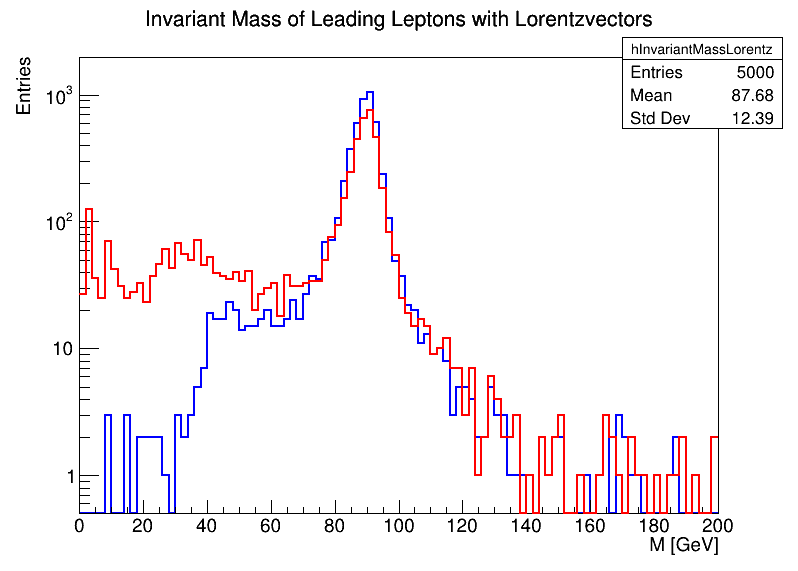
\includegraphics{Measurements/invariant_mass_comp_MC_log1.png}}
    \end{subfigure}
        \caption{\small Leading lepton's invariant mass of measured data (red) compared to the invariant mass of Monte Carlo simulation of $Z\to e^-\,e^+$ (blue). The invariant mass was computed using calculated ROOT's \texttt{TLorentzVector} class.}
        \label{fig:inv_mas}
\end{figure}

After these two observations it is clear that the preselected data has to filtered out to leave only the relevant Drell-Yan processes. For this purpose we impose isolation requirements to the measured data sets. To keep track of how many events are discarded by each applied criteria we plot a so called cut flow diagram in Figure \ref{fig:selected_events}. Additionally, we plot the invariant mass distribution of the filtered data. We do this for $Z$ process with $e$, $\mu$ or $\tau$ pairs as final state. These plots are presented in Fig \ref{fig:results_selected_data}. 

The bins on the cut-flow histogram represent applied isolations requirement. These constrains are applied consecutively from left to right. The y-axis shows the remaining number of events after the requirement on the x-axis was applied. Due to already harshly filtered data which is being used, no major change is generated by the first three conditions. For the same reason, there is no decrease in the number of events in the case of $\tau$ when Tight ID is applied. The number of events is unchanged between Lepton PDGID and Opposite Charges. For the case of $\tau$, Trigger Fired was omitted, since the data lacks a \texttt{trigT} attribute. For the Isolation requirement we apply an isolation of 0.1. 

From the cut flow histograms it is clear that the Lepton PDGID and Isolation requirements generate the biggest decrease in number of events. We conclude that cut on lepton-level constrains are more efficient than cut at event-level. Lepton-level cuts are specialized for the process to be analysed and thus are more efficient to filter out undesired events. 

The corrected mass distributions from $e$ and $\mu$ now show a prominent resonance peak around the expected mass of the $Z$ boson. In contrast, the events filtered as $\tau$ show an asymmetric distribution which tends to $\sim\SI{80}{\giga\electronvolt}$. The reason for this behaviour is the is due to the properties of $\tau$. Since these particles are unstable, they don't reach the detector and decay into other particles. Hence, the filtered events contain the leptons coming from $\tau$ decays and don't give high quality information to study the $Z$ boson. These kind of events could be identified by the $p_T$ of the resulting neutrinos, $\nu_{e/\mu}$ and $nu_\tau$, if these were able to be measured, which ATLAS is not capable of. 


\begin{figure}[htbp]
    \centering
    % First row
    \begin{subfigure}{0.45\textwidth}
        \centering
        \resizebox{0.8\textwidth}{!}{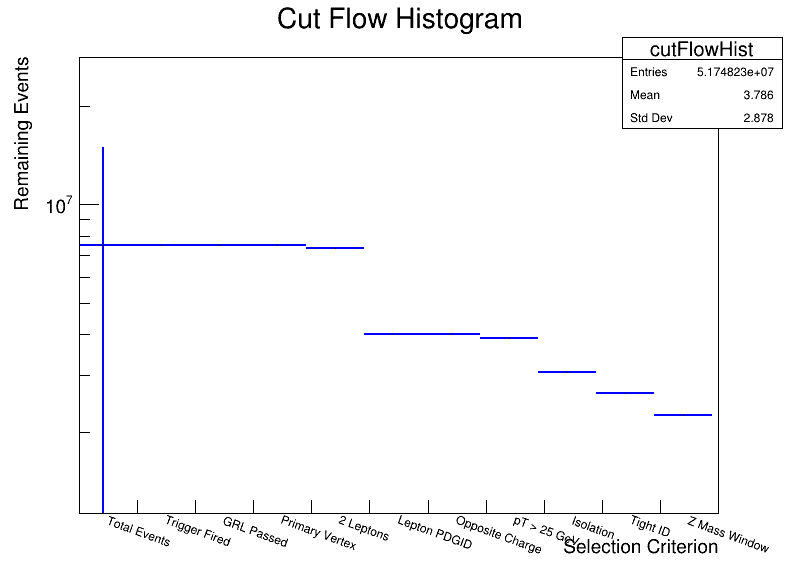
\includegraphics{Measurements/ZeecutFlowHist.png}}
    \end{subfigure}
    \hfill
    \begin{subfigure}{0.45\textwidth}
        \centering
        \resizebox{0.8\textwidth}{!}{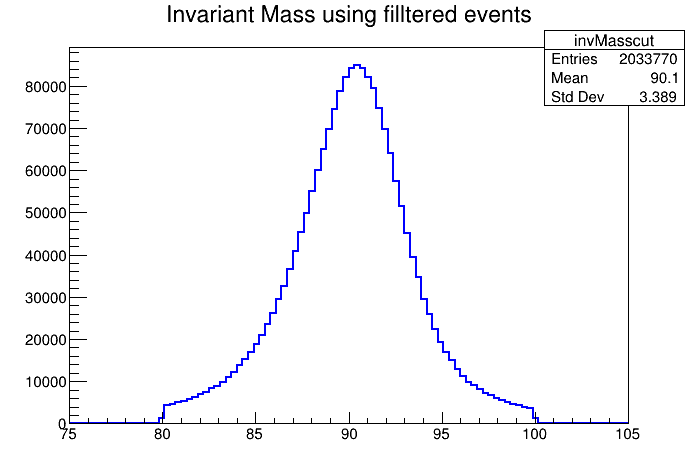
\includegraphics{Measurements/ZeeinvMass_cut.png}}
    \end{subfigure}
\vspace{1em}
    \begin{subfigure}{0.45\textwidth}
        \centering
        \resizebox{0.8\textwidth}{!}{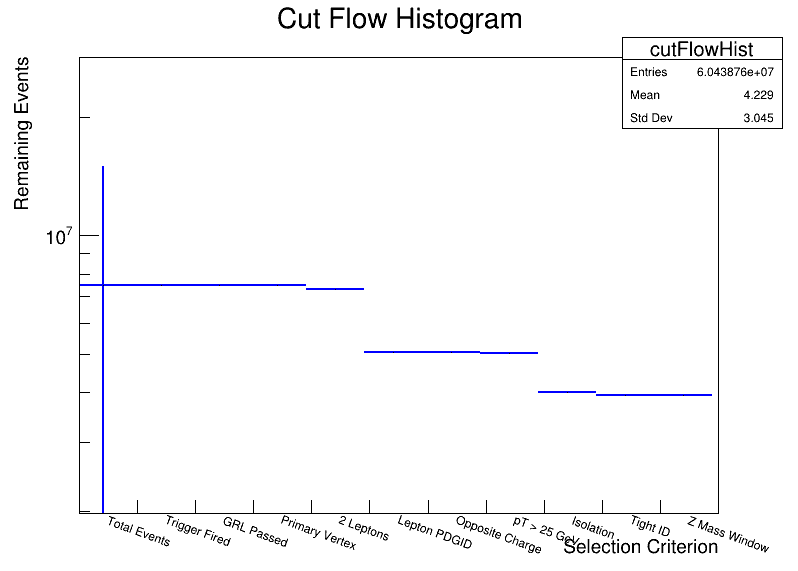
\includegraphics{Measurements/ZmumucutFlowHist.png}}
    \end{subfigure}
    \hfill
    \begin{subfigure}{0.45\textwidth}
        \centering
        \resizebox{0.8\textwidth}{!}{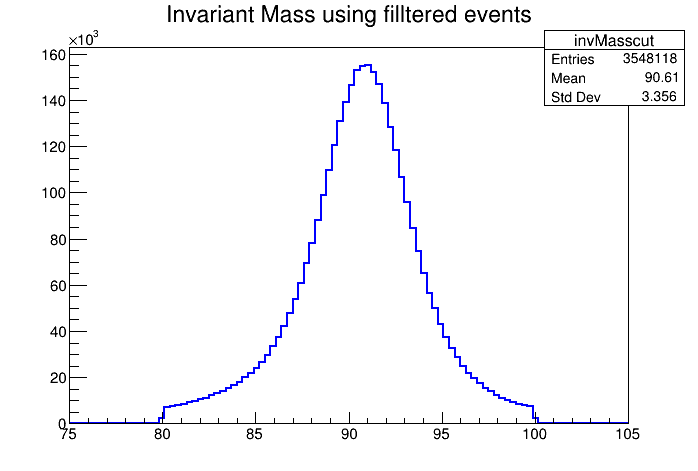
\includegraphics{Measurements/ZmumuinvMass_cut.png}}
    \end{subfigure}
\vspace{1em}
    \begin{subfigure}{0.45\textwidth}
        \centering
        \resizebox{0.8\textwidth}{!}{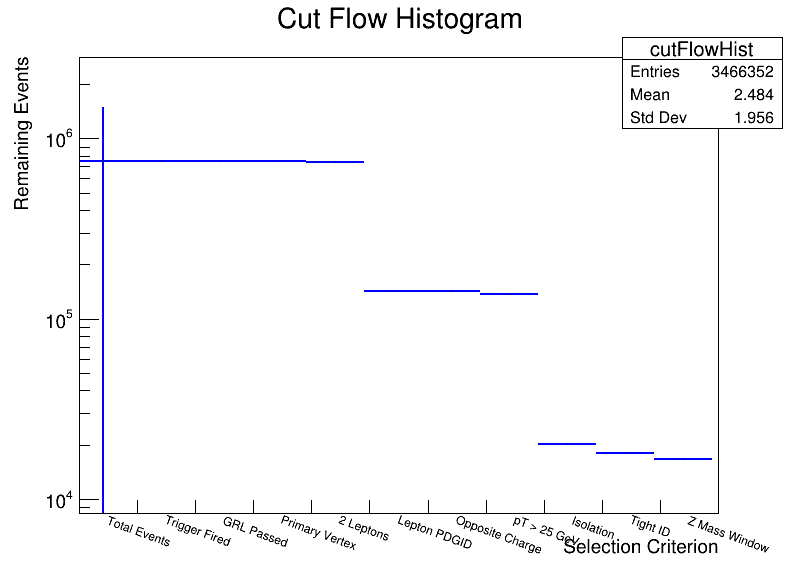
\includegraphics{Measurements/ZtautaucutFlowHist.png}}
    \end{subfigure}
    \hfill
    \begin{subfigure}{0.45\textwidth}
        \centering
        \resizebox{0.8\textwidth}{!}{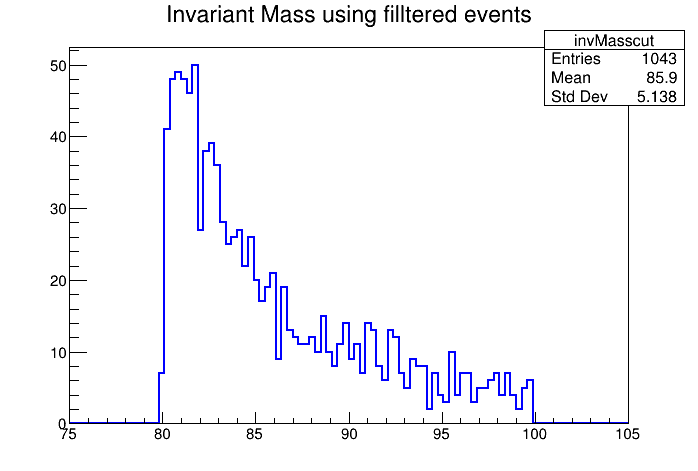
\includegraphics{Measurements/ZtautauinvMass_cut.png}}
    \end{subfigure}
    \caption{\small Cut flow from $e$, $\mu$ and $\tau$ events and invariant mass distribution of filtered data. Each row corresponds to the plots of each lepton: first row $e$, the second row $\mu$ and the third  $\tau$. The cut flow histogram is displayed on the first column and the invariant mass distribution on the left.}
    \label{fig:selected_events}
\end{figure}
\begin{figure}[htbp] 
    \centering
    % First row
    \begin{subfigure}{0.45\textwidth}
        \centering
        \resizebox{1.0\textwidth}{!}{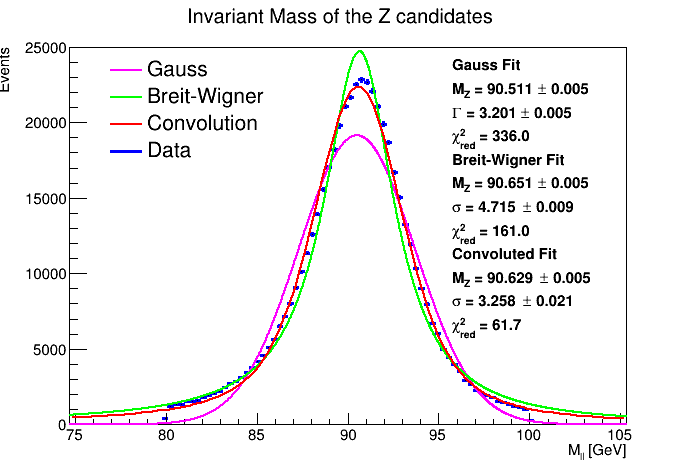
\includegraphics{Measurements/Fit.png}}
    \end{subfigure}
    \hfill
    \begin{subfigure}{0.45\textwidth}
        \centering
        \resizebox{1.0\textwidth}{!}{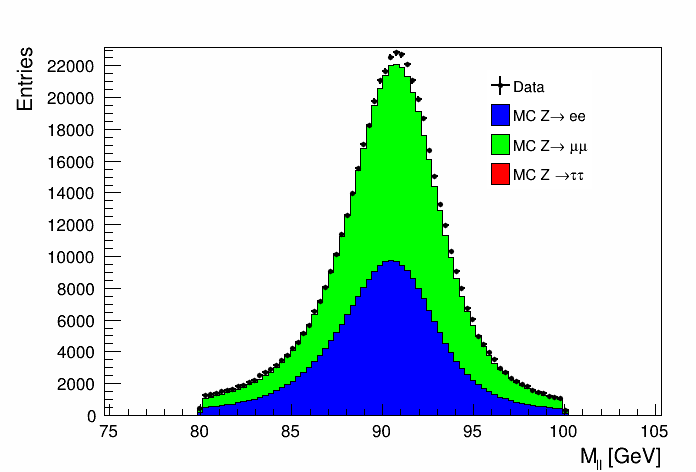
\includegraphics{Measurements/Plot.png}}
    \end{subfigure}
\vspace{1em}
    \caption{\small Right: Selected data (blue) and the fit of three distributions: (violet) Gauss-distribution, (green)Breit-Wigner Distribution and (red) convolution of a Gauss and Breit-Wigner distribution. Left: Merge of filtered electron and muon pair events  (black cross) compared to MC simulations for $Z\to l\,\bar{l}$ processes.}
    \label{fig:results_selected_data}
\end{figure}
To study the properties of the $Z$ boson we will only consider the $e$ and $\mu$ pair events. For this reason we merge the filtered $Z\to e^-e^+$ and $Z\to \mu\bar{\mu}$ events into a single histogram and compare it to the invariant mass distribution of the MC simulations, see right image in Fig. \ref{fig:results_selected_data}. The plot demonstrates the great agreement between the measured events and the MC simulations. 

Next, we compare the fit of a Gauss distribution, a relativistic Breit-Wigner (BW) distribution and the resulting distribution from the convolution of the former ones. On one hand, due to the large number of data points in our data set and the nature of the measured events, the central limit theorem dictates that the distribution of the measurements tends to a normal distribution. On the other hand, from QFT we know that the mass distribution of an unstable particles in vacuum can accurately be described by a relativistic Breit-Wigner distribution. The left image in Fig. \ref{fig:results_selected_data} makes clear that the BW renders a better fit compared to the gaussian fit. Nevertheless the $\chi^2/$dof is rather high. The convolution of both distribution shows a clear advantage over the individual fits, since it take into consideration the statistical and physical nature of the measured data. 

From the fitted convolution, we are able to determine the mass of the $Z$ boson and its width. The experimentally found values are presented in Tab. \ref{tab:results_literatur} along with the values reported by the Particle Data Group \footnote{S. Navas et al. (Particle Data Group), Dec. 2024.\href{https://pdglive.lbl.gov/Particle.action?node=S044&init=0}{[Online]}}. Even with the convolution yielding a better fit than any single distribution, we notice that the resulting mass and width for the $Z$ boson deviate significantly when compared to the values reported by PDG. We will discuss possible error sources in the discussion.

\begin{table}[!htbp]
 \begin{center}
  \caption{Comparison of measured quantities with values reported by the Particle Data Group (PDG).}
  \label{tab:results_literatur}
  \begin{tabular}{|c||c|c|c|}
  \hline
		  										& PDG 					& Fit parameter  & Deviation\\
		  										\hline
		  										\hline
  $M_Z$ [\unit{\giga\electronvolt}] & $\num{90.629\pm 0.005}$	& $\num{91.1880\pm 0.0020}$ & 27.11\\
  $\Gamma$ [\unit{\giga\electronvolt}]& $\num{3.258\pm 0.021}$ & $\num{2.4955\pm 0.0023}$&36.09\\
  \hline

\hline 
  \end{tabular}
 \end{center}
\end{table}

As a final part of our analysis we use the tag-and-probe method to determine the efficiency of the different isolation requirements used for the selection of the data. Using the characteristic signature of $ Z \rightarrow ee$ decays, the tag-and-probe method aims to produce a clean and unbiased sample to deduce said efficiency.

We introduce tight constraints upon one of the two electrons produced by the decay, in a simmilar fashion to the cut flow. The electron upon which these constraints are bestowed is the 'tag'. If it complies with the set restrictions, the second electrons, or the 'probe', will be further considered. Previous criteria on the invariant mass do still hold true and aim to further reduce background.

The efficiency is then obtained via the fraction of probe candidates that satisfy all criteria. The results of this analysis is depicted in Fig.\ref{fig:detection_Efficiency} against $p_T$.

% TODO
\begin{figure}[htbp]
    \centering
    % First row

        \centering
        \resizebox{0.5\textwidth}{!}{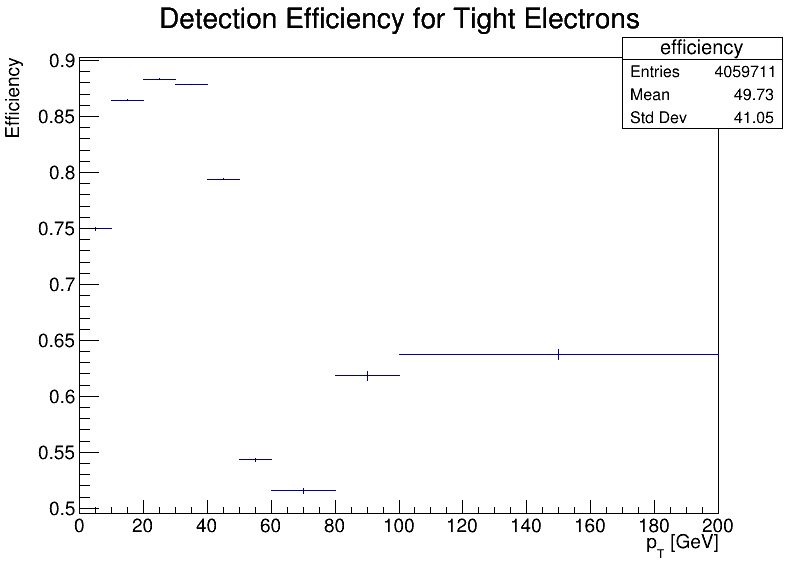
\includegraphics{Measurements/tight_Zee_efficiency.png}}
    \caption{Detection Effiency for tight Electrons obtained via the Tag-and-Probe method.}
    \label{fig:detection_Efficiency}
\end{figure}

\section{Summary}
In this experiment we examined a dataset provided by CERN from the ATLAS Detector, that was recorded in 2012 and attempted to calculate the Mass of the $Z$-Boson using the ROOT software framework, also provided by CERN.

We familiarized ourselves with the basics of ROOT's python frontend und functionalities like the TBrowser while exploring the plethora of available variables provided in the dataset.
We specifically looked at the distributions of the numbers of leptons produced, z-Position of the primary vertex, tranverse momentum, pseudorapidity and azimuthal angle observed in the collisions.

Limiting ourselves to two lepton events, we calulated the invariant mass using our own approach and using the provided TLorentzVectors, the results of which do match, but are easier to obtaine via the methods provided by ROOT.
The distribution of the Invariant Mass was further compared to Monte Carlo simulations, revealing additional resonance curves below the expected peak of $\sim 91.187GeV$, corresponding to bottom and charm resonances which likely decayed into leptons. 

To limit our data to the relevant Drell-Yan process we imposed isolation requirements upon the data like a Good run list, electron/muon trigger, restrictions on charge and so on. The effect of which can be observed in the cut flow histogram \ref{fig:selected_events}, isolating the relevant data greatly for $e$ and $\mu$ events. 

A convolution of a Breit-Wigner distribution and a Gauss distribution, was then fitted on the further selected data, yielding the final results of: $M_{z} = 92.1880 GeV$ and $\Gamma = 2.4955 GeV$, compared to the values provided by the Particle Data Group (PDG): $M_{Z,PDG} = 90.629 GeV$ and $\Gamma_{PDG} = 3.258$, we observe significant deviations of: $\sigma_{M_Z} = 27.11$ and $\sigma_{\Gamma}=36.09$.

 Lastly we had a brief examination of the efficiency using the tag and probe method. Implementing a similar routine to the cut flow specifically for the $Z \rightarrow e e$ decay, where the tag electron was subject to strict selection criteria, and if complient, the complementary probe electron was measured. This yielded the Fig.\ref*{fig:detection_Efficiency}.
 
 A discussion of the systematic errors, and deviations from expected results was undertaken in the critical discussion.
 
 

 
\section{Critical discussion}
Considering the sheer amount of effort that is put into the construction, maintanance and operation of the LHC, and the consideration of errors, addressing these is not an easy task. The preselected data might already have been subject to some corrections, that we can hardly estimate. For the purposes of our analysis, we saw that not all data was relevant, or could be used due to being the result of another processes, or producing only a certain number of leptons. 
Deviations due to the utilized software are unlikely, since it is the software  provided and utilized by CERN. More directly the implementation of the cut flow, or the fit via a convolution of distributions could lead to some deviations. In our case,  the fit model does not perfectly match the peak. One could modify the BW distribution and address the positioning and (a-)symmetry of the curve.
Additionally the $e^-$ could be missing some energy due to bremsstrahlung, for which one could include further corrections.

Lastly when examining $vxp\_z$ we saw two peaks in the distribution, which were caused by ongoing calibrations in early 2012, while the public data was recorded. Thus there might be some inconsistencies within this limited dataset when compared to the data accessible by the likes of PDG.
\end{document}
